\section{Preprocessing}

The preprocessing part is in the file 'preprocessing.py'. In this file you'll find all functions used to create sub - training, validation and testing lists and the functions that are used to process the data. Since it's better to have a uniform distribution of examples, we decided that we would take a fixed number of example for each label : 2060 examples per label for training, and 206 example per label for the validation. We then create 2266 "silences" for the training and validation. Those silences are created with the background noises given in the dataset.

\subsection{Data}

We use different preprocessing of the data in order to compare or combine them. 

\begin{itemize}
    \item Mel frequency cepstrum coefficients (MFCC)
    \item Spectral subband centroid (SSC)
\end{itemize}

Both mfcc and ssc features are obtained through a python library called python speech features. Then every kind of data is normalized to zero mean and unit variance. The data is then stored into a dictionnary which maps the data (value) to it's kind (key).

\subsection{Labels}

Labels are encoded as a list of length 22 with a one at the index of the right element and zeros otherwise.

\section{Types of neural networks}

To train our networks and implement them we use the tensorflow/keras library. 

\newpage

\subsection{MLP}

\begin{figure}[h!]
    \centering
    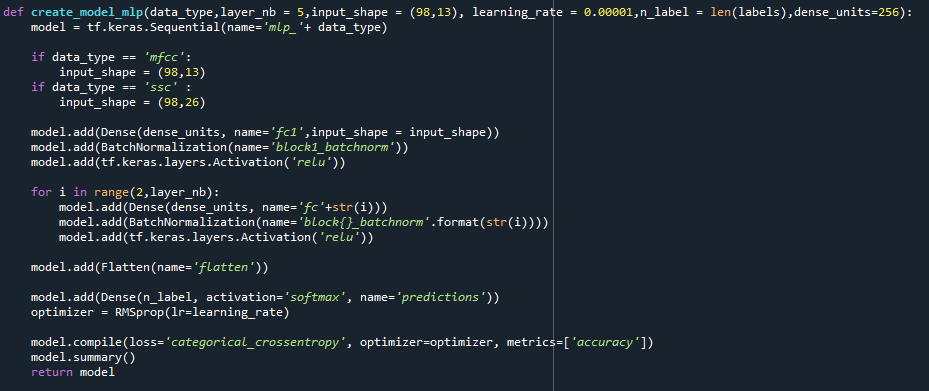
\includegraphics[width=1\textwidth]{chapters/pictures/mlp.PNG}
    \caption{Mlp structure}
    \label{fig:mlp}
\end{figure}

\subsection{CNN}
\subsubsection{Unlimited parameters CNN}

This CNN is around 24M parameters and consists of 5 convolution block with batchnorm and maxpooling. Those 5 convolutions blocks uses 64, 128, 256, 512, 512 filters. Then it uses two denses layers of 4096 neurons with a dropout of 0.5 before each layer to prevent a large overfit.

\begin{figure}[h!]
    \centering
    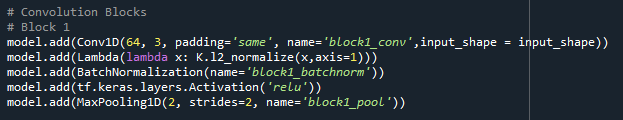
\includegraphics[width=1\textwidth]{chapters/pictures/cnn_block.PNG}
    \caption{Convolutions block}
    \label{fig:cnn_block}
\end{figure}




\begin{figure}[h!]
    \centering
    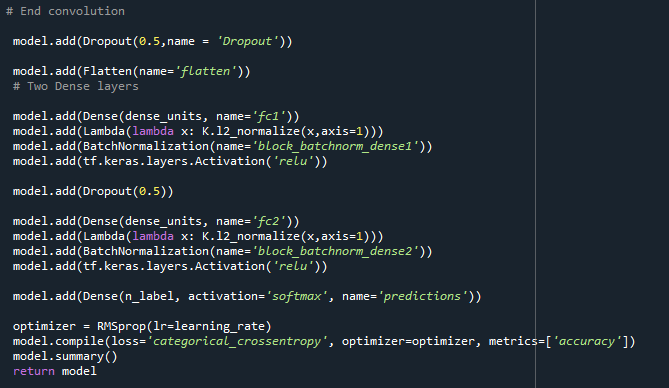
\includegraphics[width=1\textwidth]{chapters/pictures/cnn_end.PNG}
    \caption{Dense layers}
    \label{fig:cnn_end}
\end{figure}

 This makes a really heavy network that we used previously but usually able to learn whatever is asked of him. It's a good starting point. His size being around 200Mo is not extremely pratical for limited embedded devices and therefore we're looking for a smaller network.

\subsubsection{Small CNN < 250k parameters}

The idea behind this network is to try out this trend that stacks convolutions with a lower amount of pooling in a network. To keep it small we uses small numbers of filters and only one dense layer with 200 neurons. No dropout needed because of it's small size, thus we don't waste learned information and we uses the batchnorm layers power to its fullest.

\begin{figure}[h!]
    \centering
    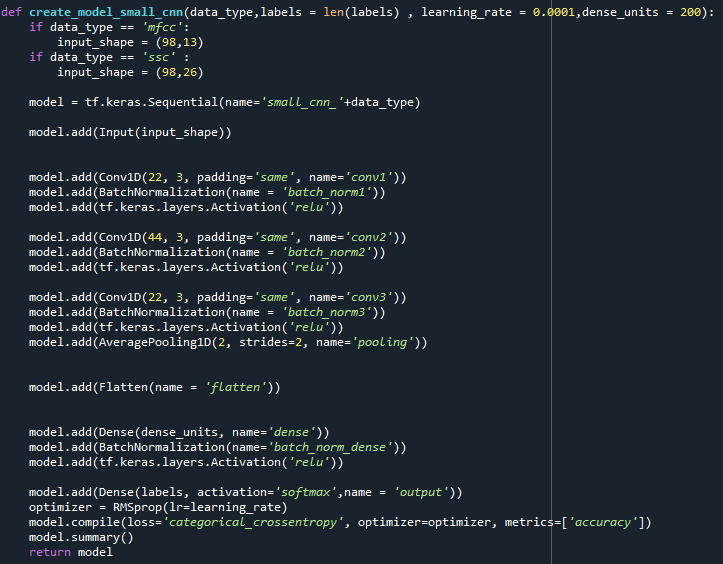
\includegraphics[width=1\textwidth]{chapters/pictures/small_cnn.PNG}
    \caption{Small CNN structure}
    \label{fig:small_cnn}
\end{figure}



\subsection{LSTM}

LSTM can be implemented with a cnn stacked on it therefore the following implementation yields two structure, one is a pure lstm and the other one is a lstm-cnn. The 

\begin{figure}[h!]
    \centering
    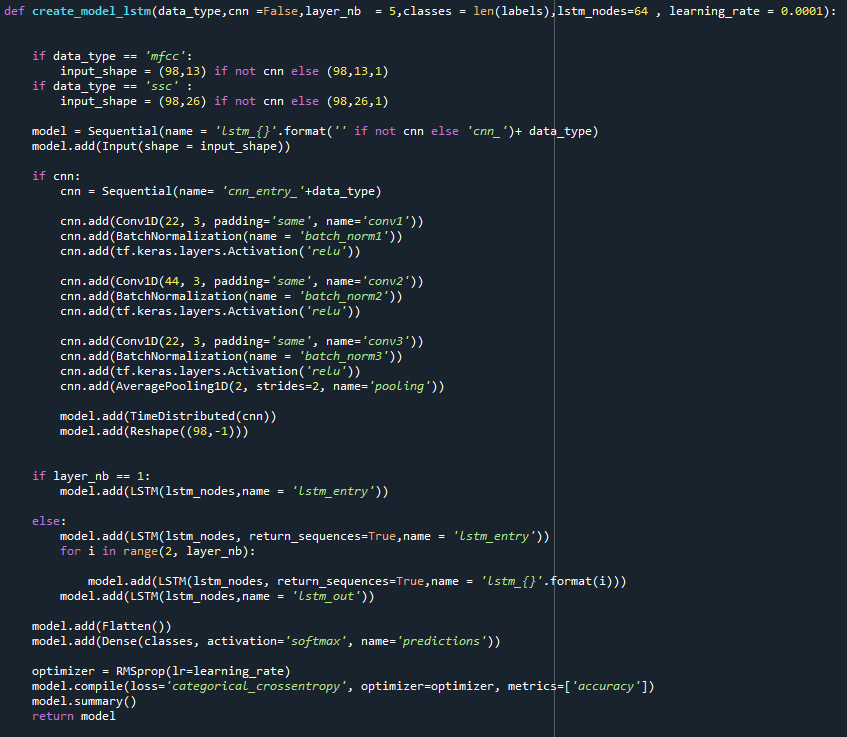
\includegraphics[width=1\textwidth]{chapters/pictures/lstm.PNG}
    \caption{Lstm structure}
    \label{fig:lstm}
\end{figure}


